\documentclass[9pt,aspectratio=169]{beamer}

\usetheme{metropolis}
\usepackage{appendixnumberbeamer}

% Font configuration
\usepackage{ifxetex,ifluatex}
\newif\ifxetexorluatex
\ifxetex\xetexorluatextrue\fi
\ifluatex\xetexorluatextrue\fi
\ifxetexorluatex
  \usepackage{fontspec}
  \usefonttheme{serif}
  \defaultfontfeatures{Ligatures=TeX}
  \setmainfont{CMU Serif}[
    UprightFont     = cmunrm.ttf,
    ItalicFont      = cmunti.ttf,
    SlantedFont     = cmunsl.ttf,
    BoldFont        = cmunbx.ttf,
    BoldItalicFont  = cmunbi.ttf,
    BoldSlantedFont = cmunbsr.ttf,  % Add this line
    Path            = /usr/share/fonts/truetype/cmu/
  ]
\fi

% Compact global sizing to fit more content
\setbeamerfont{title}{size=\Large,series=\bfseries}
\setbeamerfont{subtitle}{size=\large}
\setbeamerfont{frametitle}{size=\normalsize,series=\bfseries}
\setbeamerfont{block title}{size=\small,series=\bfseries}
\setbeamerfont{block body}{size=\scriptsize,series=\mdseries}
\setbeamerfont{caption}{size=\scriptsize}
\setbeamerfont{itemize/enumerate body}{size=\scriptsize,series=\mdseries}
\setbeamerfont{itemize/enumerate subbody}{size=\scriptsize,series=\mdseries}
\setbeamerfont{normal text}{size=\scriptsize,series=\mdseries}

% Slightly tighter lists
\setlength{\leftmargini}{1.2em}
\setlength{\leftmarginii}{1.0em}
\addtolength{\itemsep}{-0.2em}

% Optional per-slide compact mode
\newenvironment{compactslide}{%
  \begingroup
  \setbeamerfont{block body}{size=\scriptsize}%
  \setbeamerfont{itemize/enumerate body}{size=\scriptsize}%
  \setlength{\leftmargini}{1.0em}%
  \setlength{\leftmarginii}{0.8em}%
  \addtolength{\itemsep}{-0.2em}%
}{\endgroup}

% Professional color scheme with orange accents
\usepackage{amssymb,xcolor}
\definecolor{primaryOrange}{RGB}{230,126,34}
\definecolor{darkOrange}{RGB}{211,84,0}
\setbeamercolor{itemize item}{fg=primaryOrange}
\setbeamercolor{itemize subitem}{fg=darkOrange}
\setbeamercolor{alerted text}{fg=primaryOrange}
\setbeamercolor{block title}{bg=primaryOrange!15,fg=black}
\setbeamercolor{block body}{bg=primaryOrange!5}

% Professional bullet points
\setbeamertemplate{itemize item}{{\usebeamercolor[fg]{itemize item}\raisebox{0.15ex}{\small$\blacktriangleright$}}}
\setbeamertemplate{itemize subitem}{{\usebeamercolor[fg]{itemize subitem}\raisebox{0.1ex}{\footnotesize$\triangleright$}}}

% Enhanced footer
\setbeamertemplate{footline}{%
  \begin{beamercolorbox}[wd=\textwidth, sep=2ex]{footline}%
    \usebeamerfont{page number in head/foot}%
    \insertauthor\hspace{0.5em}$\cdot$\hspace{0.5em}UM6P College of Computing
    \hfill%
    \ifnum\insertframenumber=1
      \relax
    \else
      \ifnum\insertframenumber=2
        1/9
      \else
        \ifnum\insertframenumber=3
          2/9
        \else
          \ifnum\insertframenumber=4
            3/9
          \else
            \ifnum\insertframenumber=5
              4/9
            \else
              \ifnum\insertframenumber=6
                5/9
              \else
                \ifnum\insertframenumber=7
                  6/9
                \else
                  \ifnum\insertframenumber=8
                    7/9
                  \else
                    \ifnum\insertframenumber=9
                      8/9
                    \else
                      \ifnum\insertframenumber=10
                        9/9
                      \else
                        \insertframenumber/\inserttotalframenumber
                      \fi
                    \fi
                  \fi
                \fi
              \fi
            \fi
          \fi
        \fi
      \fi
    \fi
  \end{beamercolorbox}%
}

% Professional packages
\usepackage{booktabs,graphicx,tikz}
\usepackage{pgfplots}
\usepackage{xspace}
\pgfplotsset{compat=1.17}

% Custom commands for consistency
\newcommand{\separator}{\vspace{0.3em}\textcolor{primaryOrange}{\rule{\linewidth}{0.5pt}}\vspace{0.3em}}
\newcommand{\factmodel}{\textsc{FACT}\xspace}

% -------------------- Metadata --------------------
\title{Boundary-Aware \factmodel: Explicit Boundary Supervision for Frame--Action Cross-Attention}
\subtitle{SICS-155 Surgical Phase Recognition Challenge - Team AtlasVision}
\date{2025}
\author{Yasser El Jarida \and Youssef Iraqi \and Loubna Mekouar}
\institute{College of Computing, University Mohammed VI Polytechnic\\Benguerir, Morocco}

\begin{document}

% Custom title page with logos
\begin{frame}[plain]
  \begin{columns}[T,onlytextwidth]
    \column{0.7\textwidth}
      \titlepage
      \vspace{0.5em}
      {\scriptsize Slides: \url{https://yasser.sh/talks/miccai_sics155/}}
    \column{0.25\textwidth}
      \vspace{2.2 cm}
      \begin{figure}[H]
        \centering
        \vspace{-1.2em}
        
\includegraphics[width=0.9\linewidth]{demo/images/um6p_logo.pdf}
      \vspace{-1.0em}
      \end{figure}
      \vspace{0.5cm}
      \begin{figure}[H]
        \centering
        \vspace{-1.2em}
        
\includegraphics[width=0.9\linewidth]{demo/images/cc-logo.pdf}
      \vspace{-1.0em}
      \end{figure}
  \end{columns}
\end{frame}



% ========================================================
% Slide 1 — Challenge Overview
% ========================================================
\begin{frame}[label=slide1]{SICS-155 Challenge Overview}
  \begin{columns}[T,onlytextwidth]
    \column{0.65\textwidth}
      \begin{block}{Challenge Details}
        \textbf{SICS-155:} 155 videos, 19 phases, 100 train / 15 test
        
        \textbf{Key Challenge:} Temporal boundary ambiguity at phase transitions
        \begin{itemize}
          \item Over-segmentation: short spurious segments
          \item Boundary blurring between adjacent actions
          \item Need for stable phase segmentation
        \end{itemize}
      \end{block}
      
      \begin{block}{Team AtlasVision Approach}
        \textbf{Strategy:} Boundary-aware training for better temporal consistency
        
        \textbf{Base Model:} \factmodel with I3D features
        
        \textbf{Innovation:} Auxiliary boundary head for transition prediction
      \end{block}
      
    \column{0.3\textwidth}
      \begin{block}{}
        \vspace{-1.5em}
        \begin{figure}[H]
          \centering
          \vspace{-1.2em}
          
\includegraphics[width=0.8\linewidth]{demo/images/miccai2025-logo.png}
          \vspace{-0.5em}
          \caption{\scriptsize MICCAI 2025}
          \vspace{-1.2em}
        \end{figure}
        \vspace{0.1em}
      \end{block}
      \vspace{-0.2cm}
      \begin{block}{}
        \vspace{-1.0em}
        \begin{figure}[H]
          \centering
          \vspace{-1.2em}
          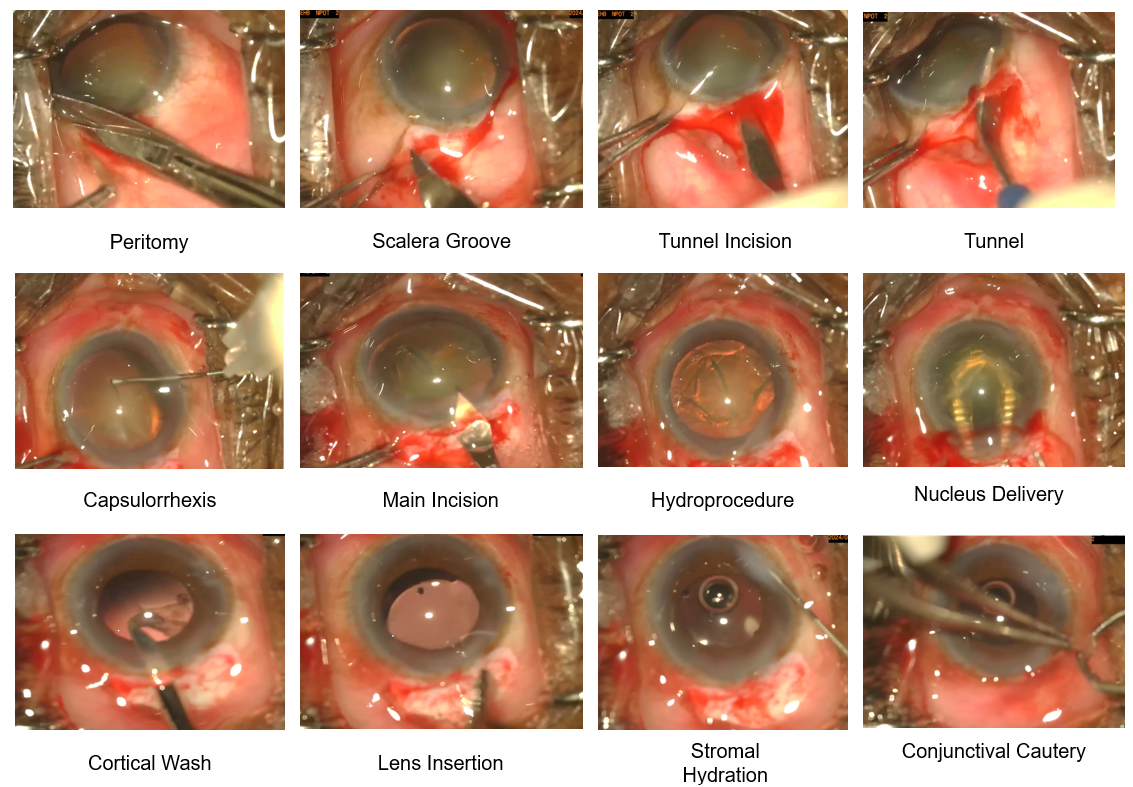
\includegraphics[width=\linewidth]{demo/images/sics155_preview.png}
          \vspace{-2.0em}
          \caption{\scriptsize SICS phases}
          \vspace{-1.2em}
        \end{figure}
        \vspace{0.1em}
      \end{block}
  \end{columns}
\end{frame}


% ========================================================
% Slide 2 — Previous Methods & Validation Results
% ========================================================
\begin{frame}[label=slide2]{Previous Methods \& Validation Results}
  \begin{columns}[T,onlytextwidth]
    \column{0.65\textwidth}
      \begin{block}{MS-TCN++ with custom features}
        \textbf{VideoMAE-v2 features:}
        \begin{itemize}
          \item Pretrain: Cataract-1K + OphNet (2024), then finetune on Cataract101
          \item Segmenter: MS-TCN++ \ (MSTCN2-style temporal convs)
          \item Outcome: lower Acc/F1/Edit; unstable early training
        \end{itemize}
        \textbf{I3D features + MS-TCN++:} improved but \textbf{< 80\% Acc}
      \end{block}

      \begin{block}{Surgformer (HTA head)}
        \begin{itemize}
          \item Microscopic + macroscopic temporal attention for long-range dependencies
          \item \textbf{Acc \~82\%} on validation, but \textbf{poor F1/Edit}
        \end{itemize}
      \end{block}

      \begin{block}{Motivation for \factmodel}
        Combine convolutional efficiency with transformer long-range modeling via cross-attention
      \end{block}

    \column{0.3\textwidth}
      \begin{block}{Notes}
        \scriptsize
        \vspace{-0.4em}
        \begin{itemize}
          \item VideoMAE-v2 + MS-TCN++ unstable from early epochs
          \item I3D + MS-TCN++ improved stability but < 80\% Acc
          \item Surgformer: long-range modeling, but weak F1/Edit
        \end{itemize}
        \vspace{-0.2em}
      \end{block}
  \end{columns}
\end{frame}

% ========================================================
% Slide 3 — Approach \& FACT Baseline
% ========================================================
\begin{frame}[label=slide3]{Approach \& \factmodel Baseline}
  \begin{columns}[T,onlytextwidth]
    \column{0.65\textwidth}
      \begin{block}{High-level approach}
        \begin{itemize}
          \item Backbone features: I3D
          \item Temporal model: \factmodel (frame CNN branch + action-token transformer)
          \item Information exchange: bidirectional cross-attention between branches
          \item Inference: merge token-derived posteriors with frame logits via a learned weight
        \end{itemize}
      \end{block}

      \begin{block}{How it works (simple view)}
        \begin{itemize}
          \item \textbf{Frame branch (convolutions):} captures local motion/appearance and produces per-frame class scores efficiently.
          \item \textbf{Action branch (tokens + transformer):} a \emph{small set of learnable action tokens} model long-range structure and segment-level context.
          \item \textbf{Cross-attention (both directions):} tokens attend to frames to align with segments; frames attend to tokens to receive high-level guidance.
          \item \textbf{Final prediction:} combine guidance from tokens with the frame branch for stable, accurate framewise labels.
        \end{itemize}
      \end{block}

    \column{0.3\textwidth}
      \begin{minipage}[c][0.75\textheight][c]{\linewidth}
        \begin{block}{}
          \begin{figure}[H]
            \centering
            \vspace{-1.0em}
            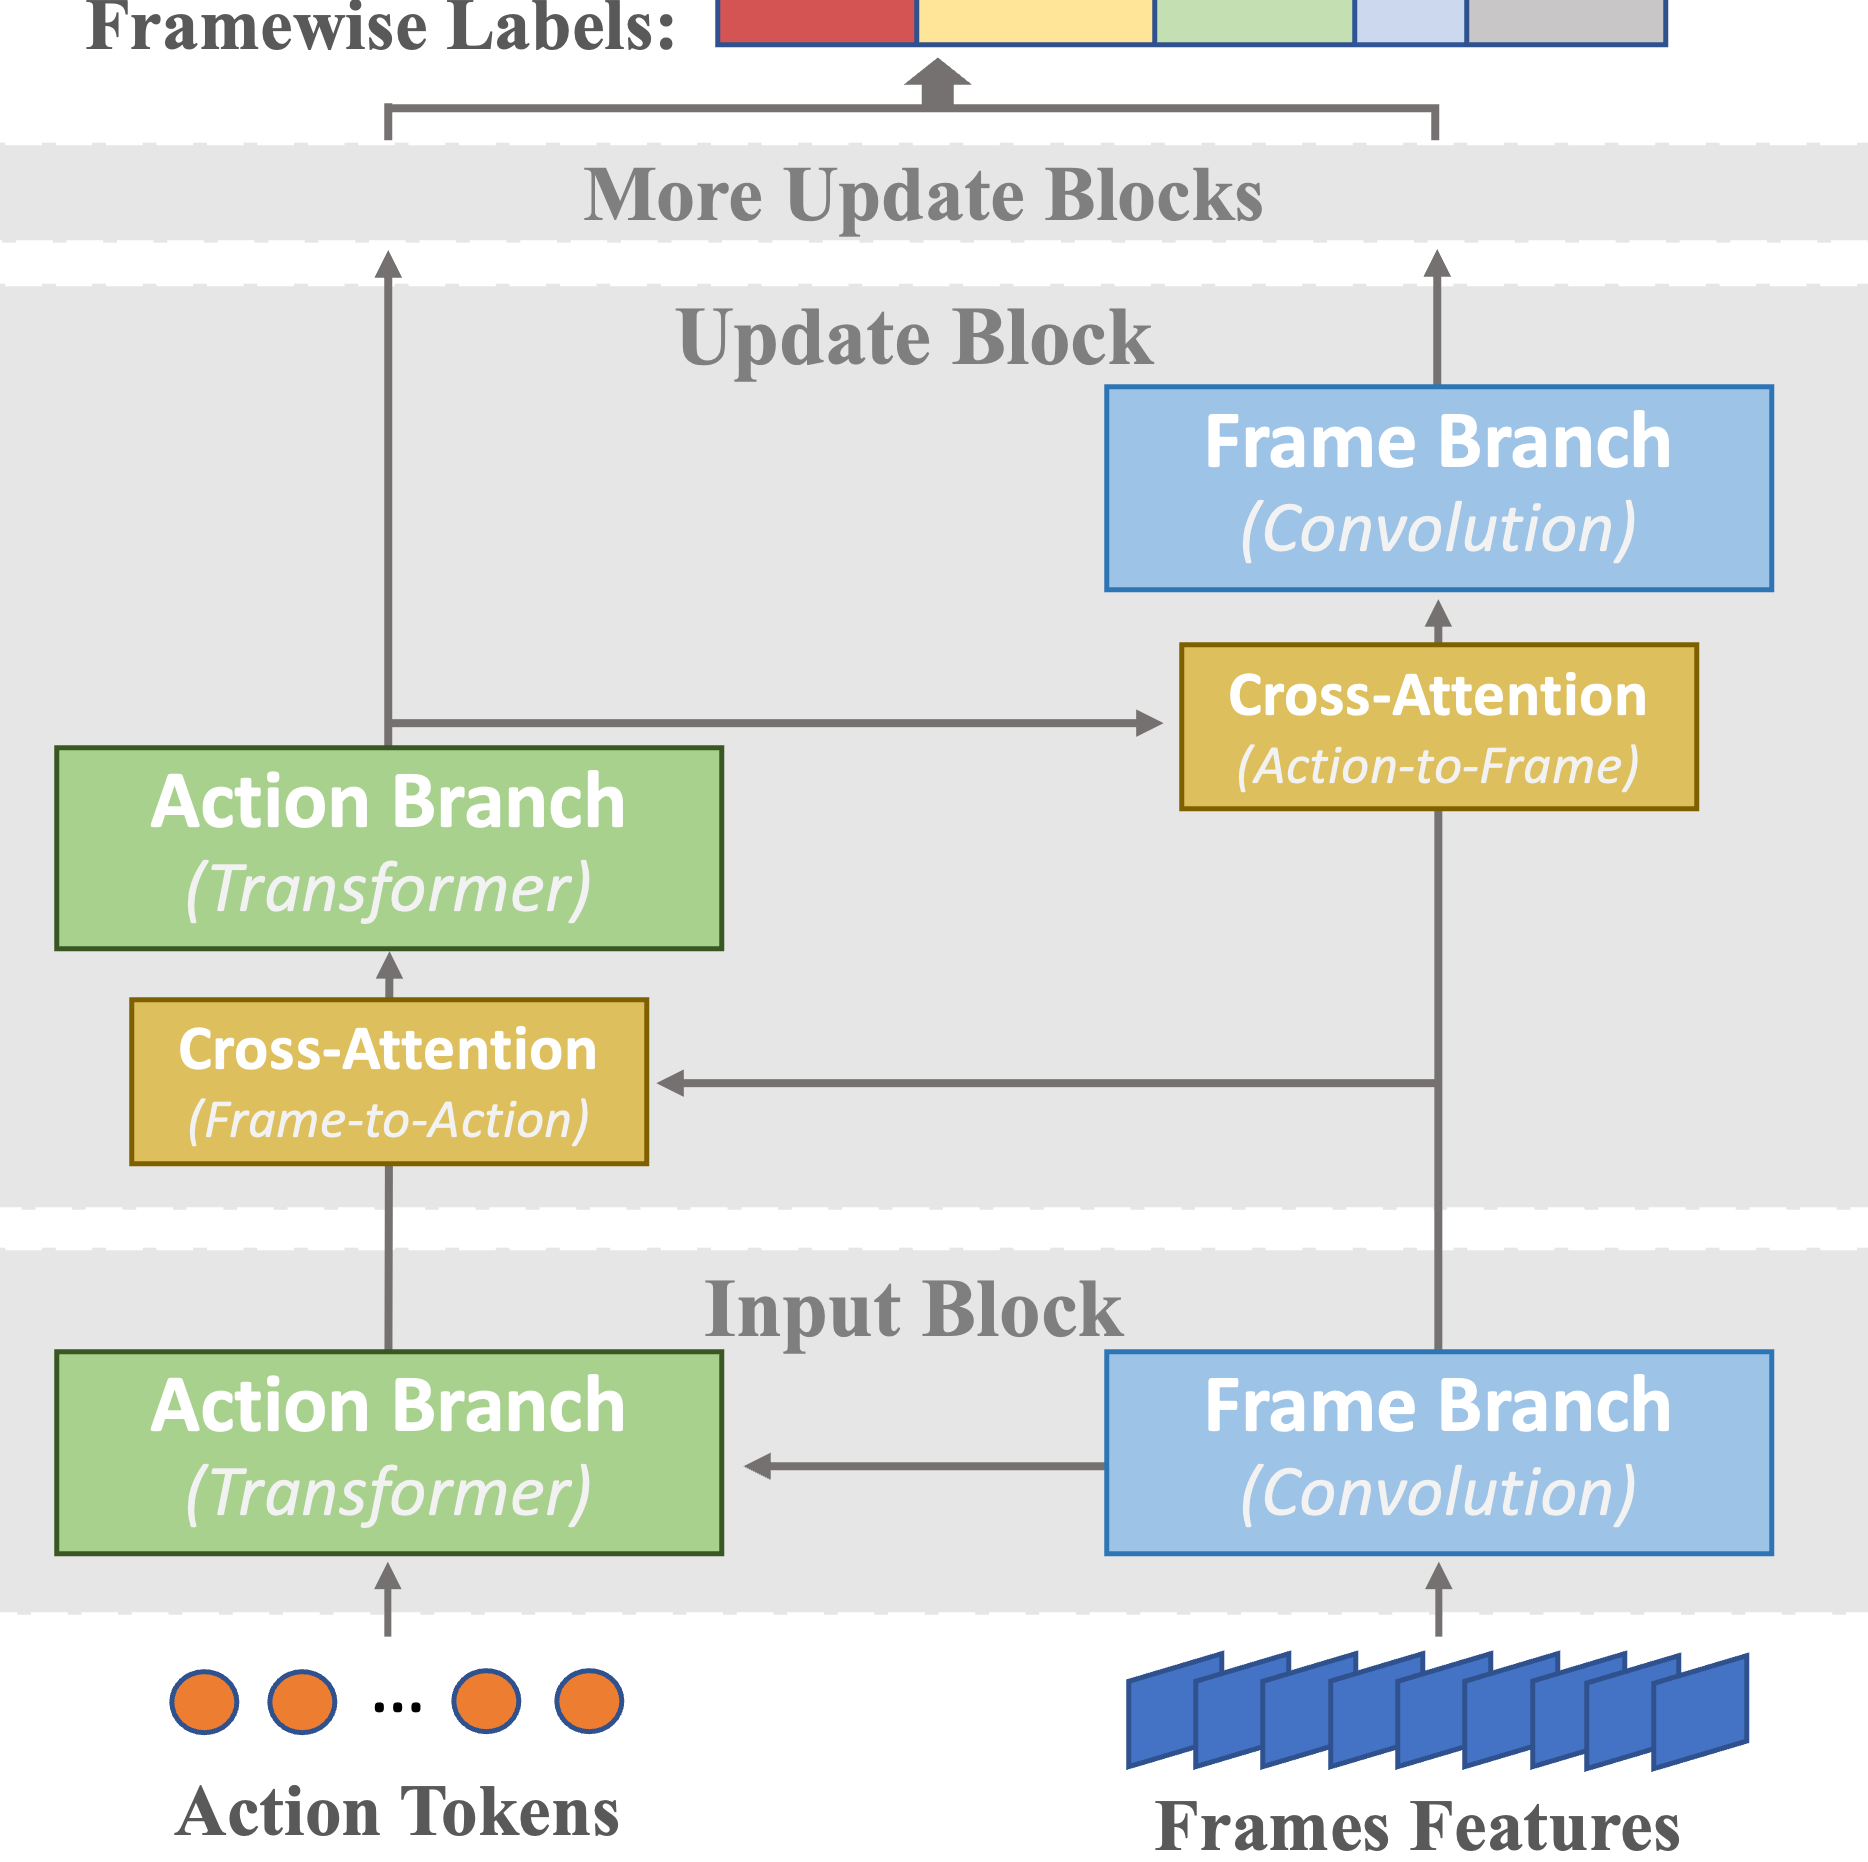
\includegraphics[width=\linewidth]{demo/images/overview.png}
            \vspace{-2.0em}
            \caption{\scriptsize \factmodel baseline}
            \vspace{-1.2em}
          \end{figure}
        \end{block}
      \end{minipage}
  \end{columns}
\end{frame}

% ========================================================
% Slide 4 — Boundary-aware Extension (Architecture \& Loss)
% ========================================================
\begin{frame}[label=slide4]{Boundary-aware Extension (Architecture \& Loss)}
  \begin{columns}[T,onlytextwidth]
    \column{0.65\textwidth}
      \begin{block}{Loss formulation}
        \textbf{Boundary detection (BCE):}
        $\displaystyle \mathcal{L}_{\text{BCE}}=\tfrac{1}{T}\sum_{t}\big(-y_b(t)\log p_b(t)-(1-y_b(t))\log(1-p_b(t))\big)$

        \textbf{Boundary-weighted TV:}
        $\displaystyle \mathcal{L}_{\text{TV}}^{\text{w}}=\frac{1}{T-1}\sum_{t=1}^{T-1}(1-p_b(t))^{\gamma}\, \|\log\mathbf{p}_{t+1}-\log\mathbf{p}_t\|_2^2$

        \textbf{Combined per-block:}
        $\displaystyle \mathcal{L}_{\text{block}}=\mathcal{L}_{\text{frame}}+\mathcal{L}_{\text{token}}+\mathcal{L}_{\text{attn}}+\alpha\,\mathcal{L}_{\text{TV}}^{\text{w}}+\beta\,\mathcal{L}_{\text{BCE}}$
      \end{block}

      \begin{block}{Intuition}
        \begin{itemize}
          \item Stabilize interiors; allow sharp changes at true transitions
          \item Gate smoothing by $(1-p_b(t))^{\gamma}$
          \item No inference cost or parameter changes
        \end{itemize}
      \end{block}
      
    \column{0.3\textwidth}
      \begin{block}{}
        \begin{figure}[H]
          \centering
          \vspace{-1.0em}
          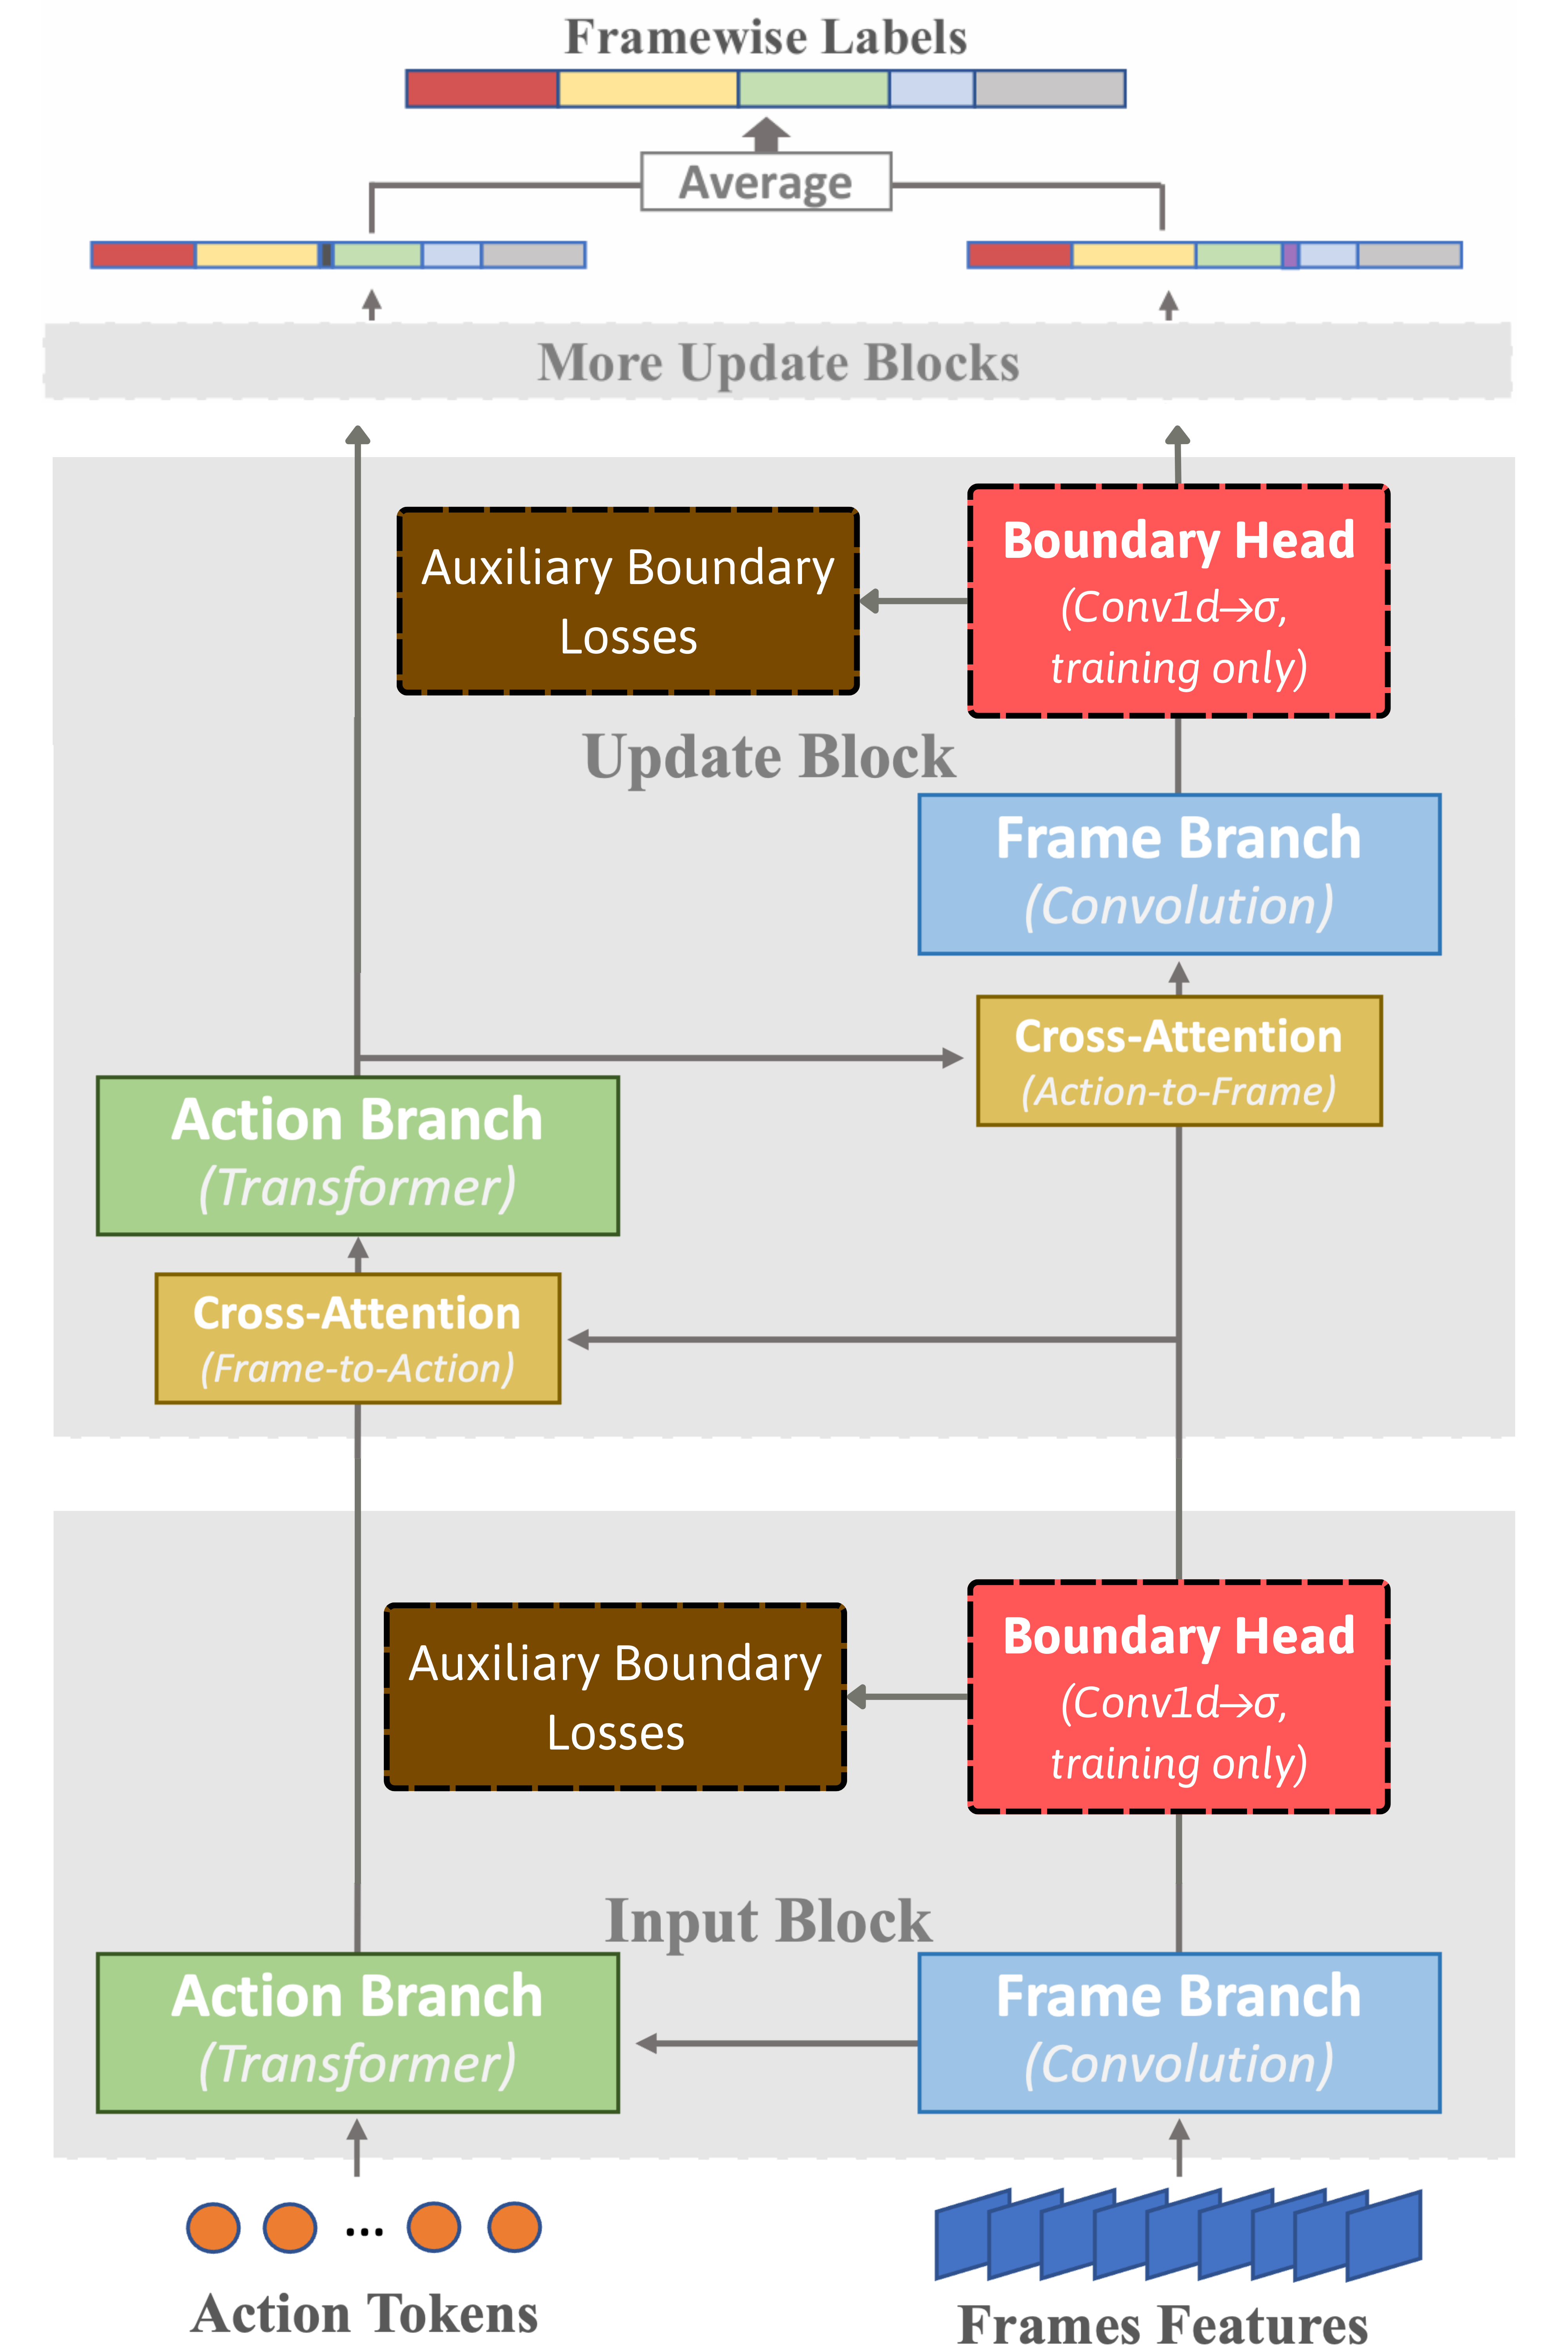
\includegraphics[width=\linewidth]{demo/images/Boundary_Head.png}
          \vspace{-2.0em}
          \caption{\scriptsize Boundary-aware head placement}
          \vspace{-1.2em}
        \end{figure}
      \end{block}
  \end{columns}
\end{frame}

% ========================================================
% Slide 5 — Experimental Setup
% ========================================================
\begin{frame}[label=slide4a]{Experimental Setup}
  \begin{columns}[T,onlytextwidth]
    \column{0.65\textwidth}
      \begin{block}{Dataset \& Features}
        \textbf{SICS-155:} 100 train / 15 test videos, 19 phases
        \begin{itemize}
          \item 960×540 resolution @ 30 FPS
          \item I3D features: 1024-D spatiotemporal embeddings
          \item Extracted at stride $sr = 3$
        \end{itemize}
      \end{block}
      
      \begin{block}{Training Strategy}
        \textbf{Warm Start:} Vanilla \factmodel baseline
        \begin{itemize}
          \item Load shared weights, initialize boundary heads
          \item Learning rate: $1 \times 10^{-4}$
          \item Merge weight: $w = 0.50$
        \end{itemize}
        
        \textbf{Hyperparameter Search:} W\&B sweeps
        \begin{itemize}
          \item Boundary loss weight: $\{1.0, 1.5, 2.0\}$
          \item TV exponent: $\{2.0, 3.0\}$
          \item Smoothing weight: $\{1.0, 2.5, 5.0\}$
        \end{itemize}
      \end{block}
      
    \column{0.3\textwidth}
      \begin{block}{Hardware}
        \begin{itemize}
          \item Single NVIDIA RTX 6000 Ada Generation GPU
          \item Efficient training with warm initialization
        \end{itemize}
      \end{block}
  \end{columns}
\end{frame}

% % ========================================================
% % Slide 5 — Previous Methods \& Validation Results
% % ========================================================
% \begin{frame}[label=slide5]{Previous Methods \& Validation Results}
%   \begin{columns}[T,onlytextwidth]
%     \column{0.65\textwidth}
%       \begin{block}{MS-TCN++ with custom features}
%         \textbf{VideoMAE-v2 features:}
%         \begin{itemize}
%           \item Pretrain: Cataract-1K + OphNet (2024), then finetune on Cataract101
%           \item Segmenter: MS-TCN++
%           \item Outcome: lower Acc/F1/Edit; unstable early training
%         \end{itemize}
%         \textbf{I3D features + MS-TCN++:} improved but \textbf{< 80\% Acc}
%       \end{block}

%       \begin{block}{Surgformer (HTA head)}
%         \begin{itemize}
%           \item Microscopic + macroscopic temporal attention for long-range dependencies
%           \item \textbf{Acc \~82\%} on validation, but \textbf{poor F1/Edit}
%         \end{itemize}
%       \end{block}

%       \begin{block}{Takeaway}
%         \factmodel balances efficiency and long-range modeling better than either family alone
%       \end{block}

%     \column{0.3\textwidth}
%       \begin{block}{}
%         \vspace{-1.0em}
%         \begin{figure}[H]
%           \centering
%           \vspace{-1.2em}
%           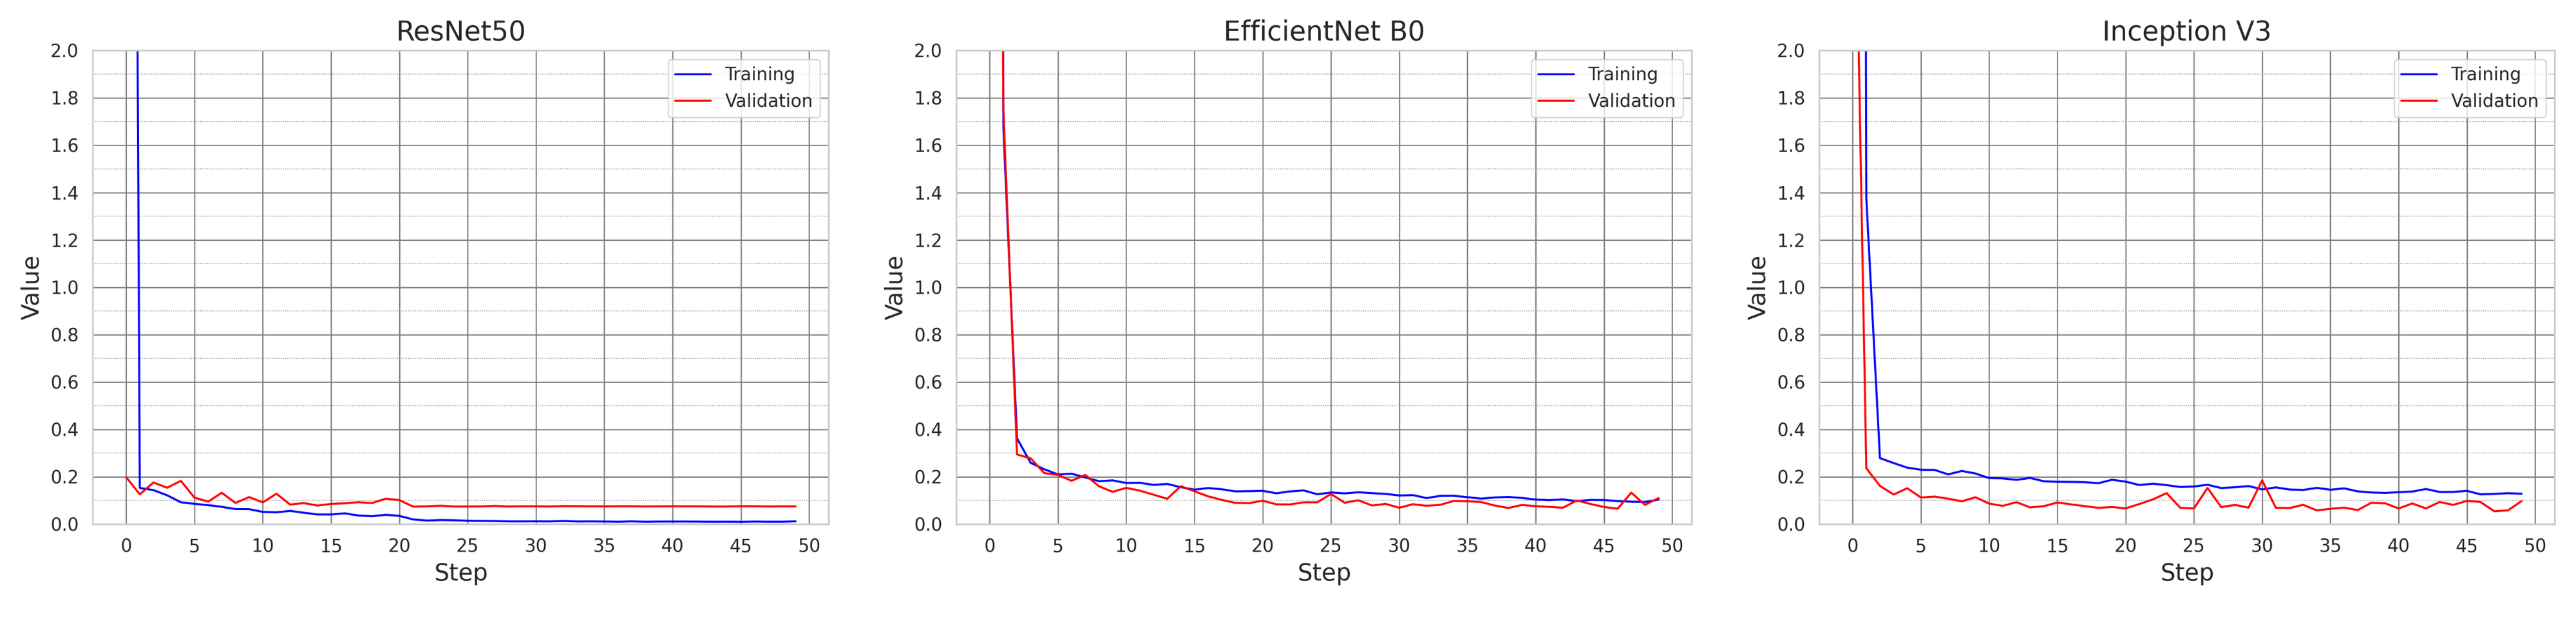
\includegraphics[width=\linewidth]{demo/images/results.png}
%           \vspace{-2.0em}
%           \caption{\scriptsize Validation trends}
%           \vspace{-1.2em}
%         \end{figure}
%         \vspace{0.1em}
%       \end{block}
%   \end{columns}
% \end{frame}

% ========================================================
% Slide 6 — Hyperparameter Tuning (W&B Sweeps)
% ========================================================
\begin{frame}[label=slide6]{Hyperparameter Tuning (W\&B Sweeps)}
  \begin{columns}[T,onlytextwidth]
    \column{0.6\textwidth}
      \begin{block}{Search spaces}
        \begin{itemize}
          \item $\beta$ (boundary BCE): $\{1.0,1.5,2.0\}$
          \item $\gamma$ (TV exponent): $\{2.0,3.0\}$
          \item $\alpha$ (smoothing): $\{1.0,2.5,5.0\}$
          \item Frame feature stride $sr$: $\{1,3,5\}$
          \item Merge weight $w$: fixed $0.50$; LR $1\times 10^{-4}$; $M=36$
        \end{itemize}
      \end{block}
      \begin{block}{Selected configuration}
        $\beta=1.0,\ \gamma=2.0,\ \alpha=5.0,\ sr=3,\ w=0.50,\ M=36$
      \end{block}
    \column{0.35\textwidth}
      \begin{block}{}
        \vspace{-0.6em}
        \centering
        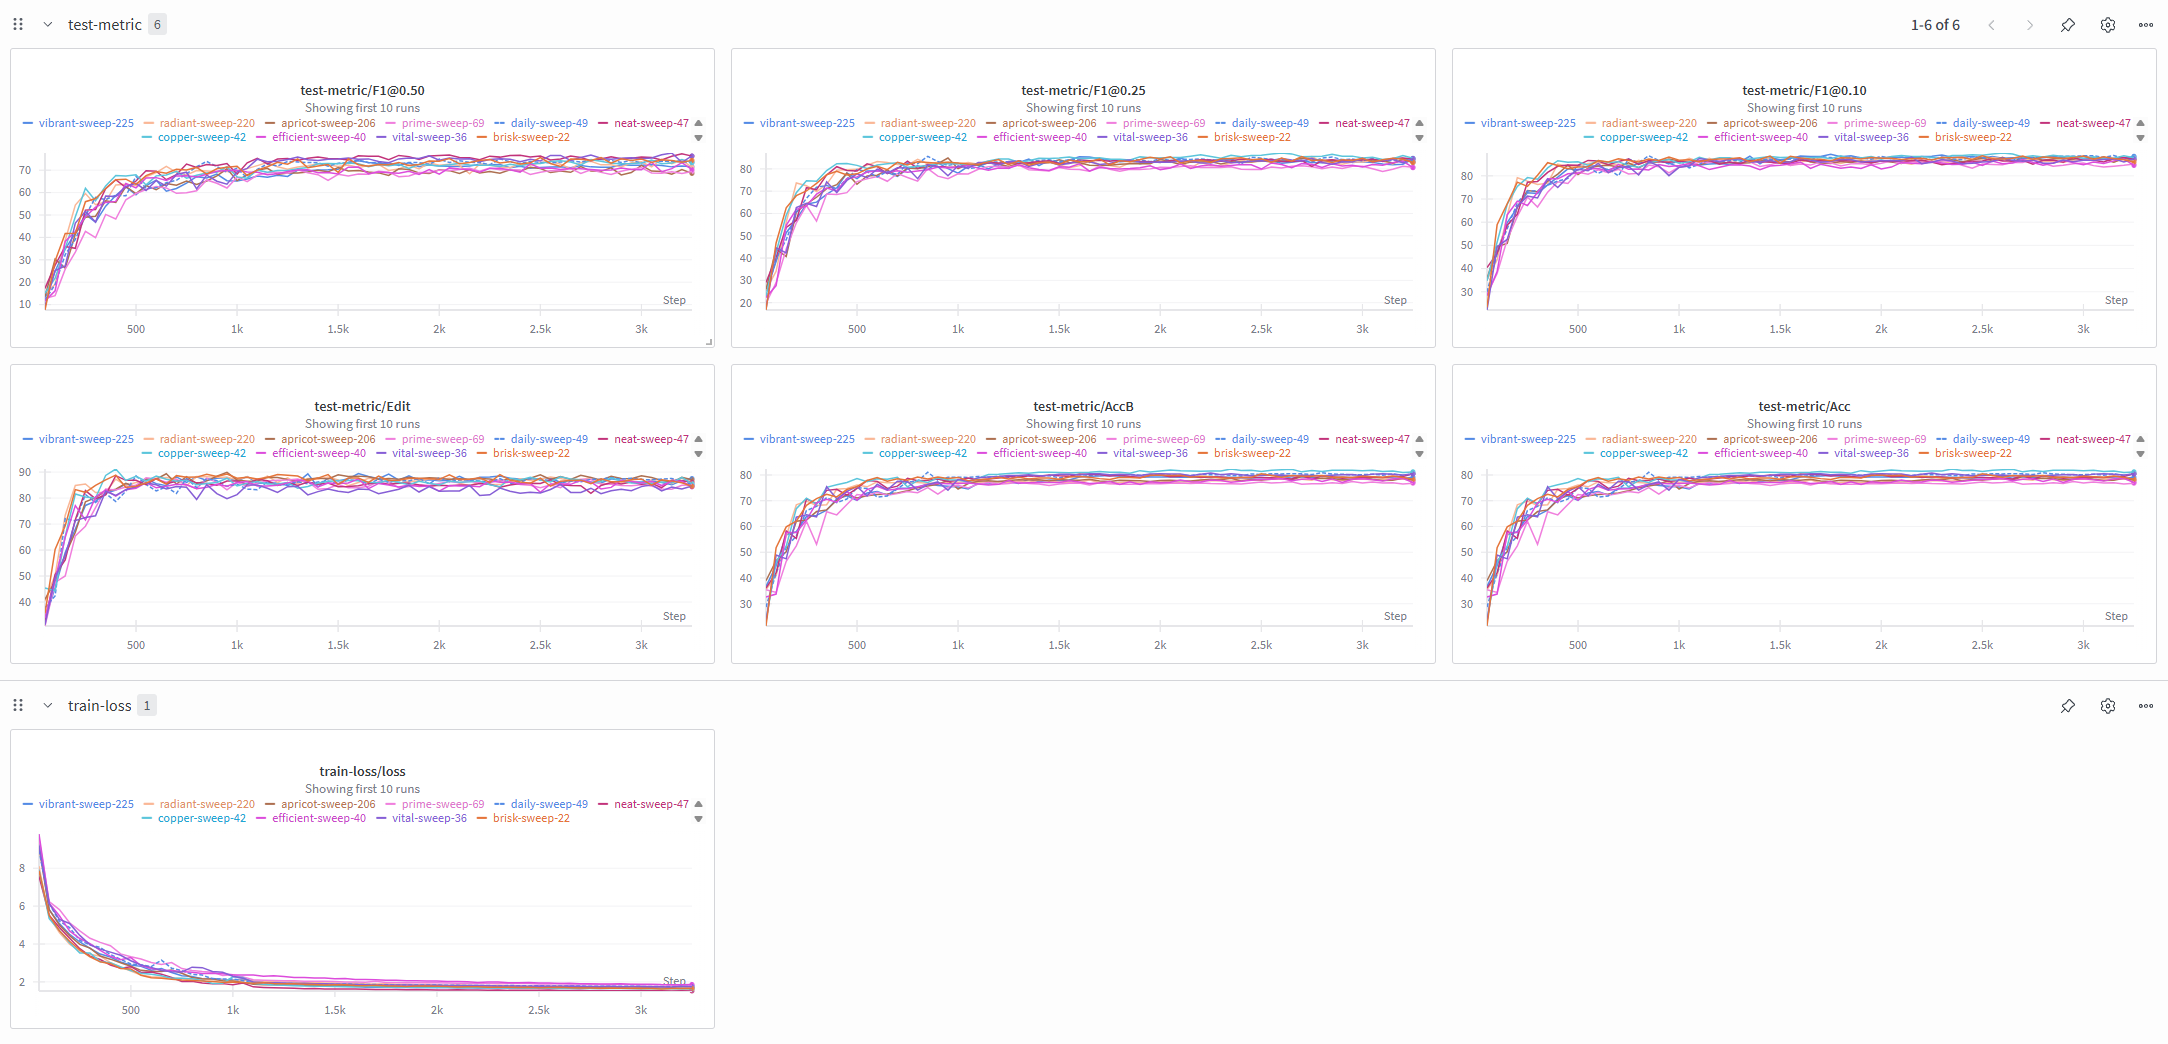
\includegraphics[width=\linewidth]{demo/images/sweep_without_boundary.png}\\[-0.2em]
        {\scriptsize w/o boundary}\\[0.4em]
        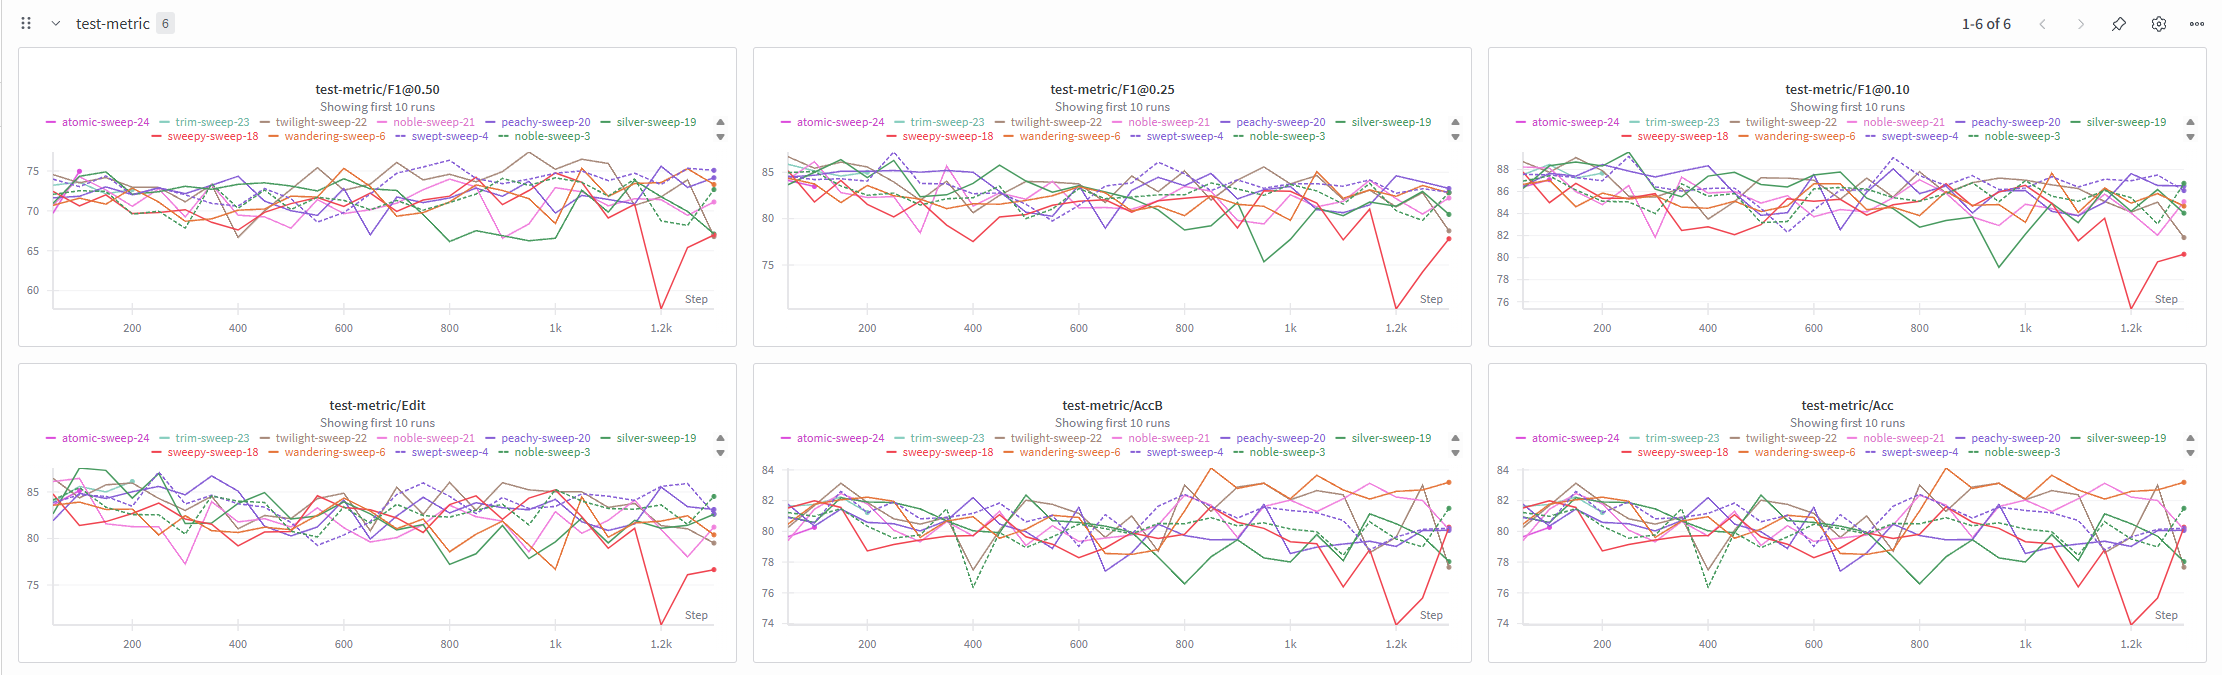
\includegraphics[width=\linewidth]{demo/images/sweep_with_boundary.png}\\[-0.2em]
        {\scriptsize with boundary (warm start)}
        \vspace{-0.6em}
      \end{block}
  \end{columns}
\end{frame}

% ========================================================
% Slide 7 — Results & Performance
% ========================================================
\begin{frame}[label=slide7]{Results \& Performance (Validation \& Test)}
  \begin{columns}[T,onlytextwidth]
    \column{0.6\textwidth}
      \begin{block}{Test Set Results}
        \textbf{SICS-155 Challenge Submission:}
        \begin{itemize}
          \item \textbf{Accuracy: 82\%} (Rank \#2 on leaderboard)
          \item Consistent performance across test videos
          \item Boundary-aware variant showed improvements
        \end{itemize}
      \end{block}
      
      \begin{block}{Validation Set (Public)}
        \vspace{0.5em}
        \centering
        \renewcommand{\arraystretch}{1.15}
        \begin{tabular}{lccc}
          \toprule
          \textbf{Method} & \textbf{Acc (\%)} & \textbf{F1@0.50} & \textbf{Edit} \\
          \midrule
          \factmodel & 82.8 & 77.1 & \textbf{86.9} \\
          + boundary & \textbf{84.1} & \textbf{78.6} & 86.3 \\
          \bottomrule
        \end{tabular}
        \vspace{0.5em}
      \end{block}
      
      \begin{block}{Qualitative Improvements}
        \begin{itemize}
          \item Cleaner phase transitions
          \item Fewer short spurious segments
          \item Better boundary adherence
        \end{itemize}
      \end{block}
      
    \column{0.35\textwidth}
      \begin{block}{Key Insights}
        \begin{itemize}
          \item Boundary awareness helps temporal consistency
          \item Minimal computational overhead
          \item Warm start crucial for stability
        \end{itemize}
      \end{block}
  \end{columns}
\end{frame}

% % ========================================================
% % Slide 7 — W&B Sweeps (Tuning)
% % ========================================================
% \begin{frame}[label=slide7]{Hyperparameter Tuning (W\&B Sweeps)}
%   \begin{columns}[T,onlytextwidth]
%     \column{0.6\textwidth}
%       \begin{block}{Search spaces}
%         \begin{itemize}
%           \item $\beta$ (boundary BCE): $\{1.0,1.5,2.0\}$
%           \item $\gamma$ (TV exponent): $\{2.0,3.0\}$
%           \item $\alpha$ (smoothing): $\{1.0,2.5,5.0\}$
%           \item Merge weight $w$: fixed $0.50$; LR $1\times 10^{-4}$; $M=36$
%         \end{itemize}
%       \end{block}
%       \begin{block}{Selected configuration}
%         $\beta=1.0,\ \gamma=2.0,\ \alpha=5.0,\ w=0.50,\ M=36$
%       \end{block}
%     \column{0.35\textwidth}
%       \begin{block}{}
%         \vspace{-1.0em}
%         \begin{figure}[H]
%           \centering
%           \vspace{-1.2em}
%           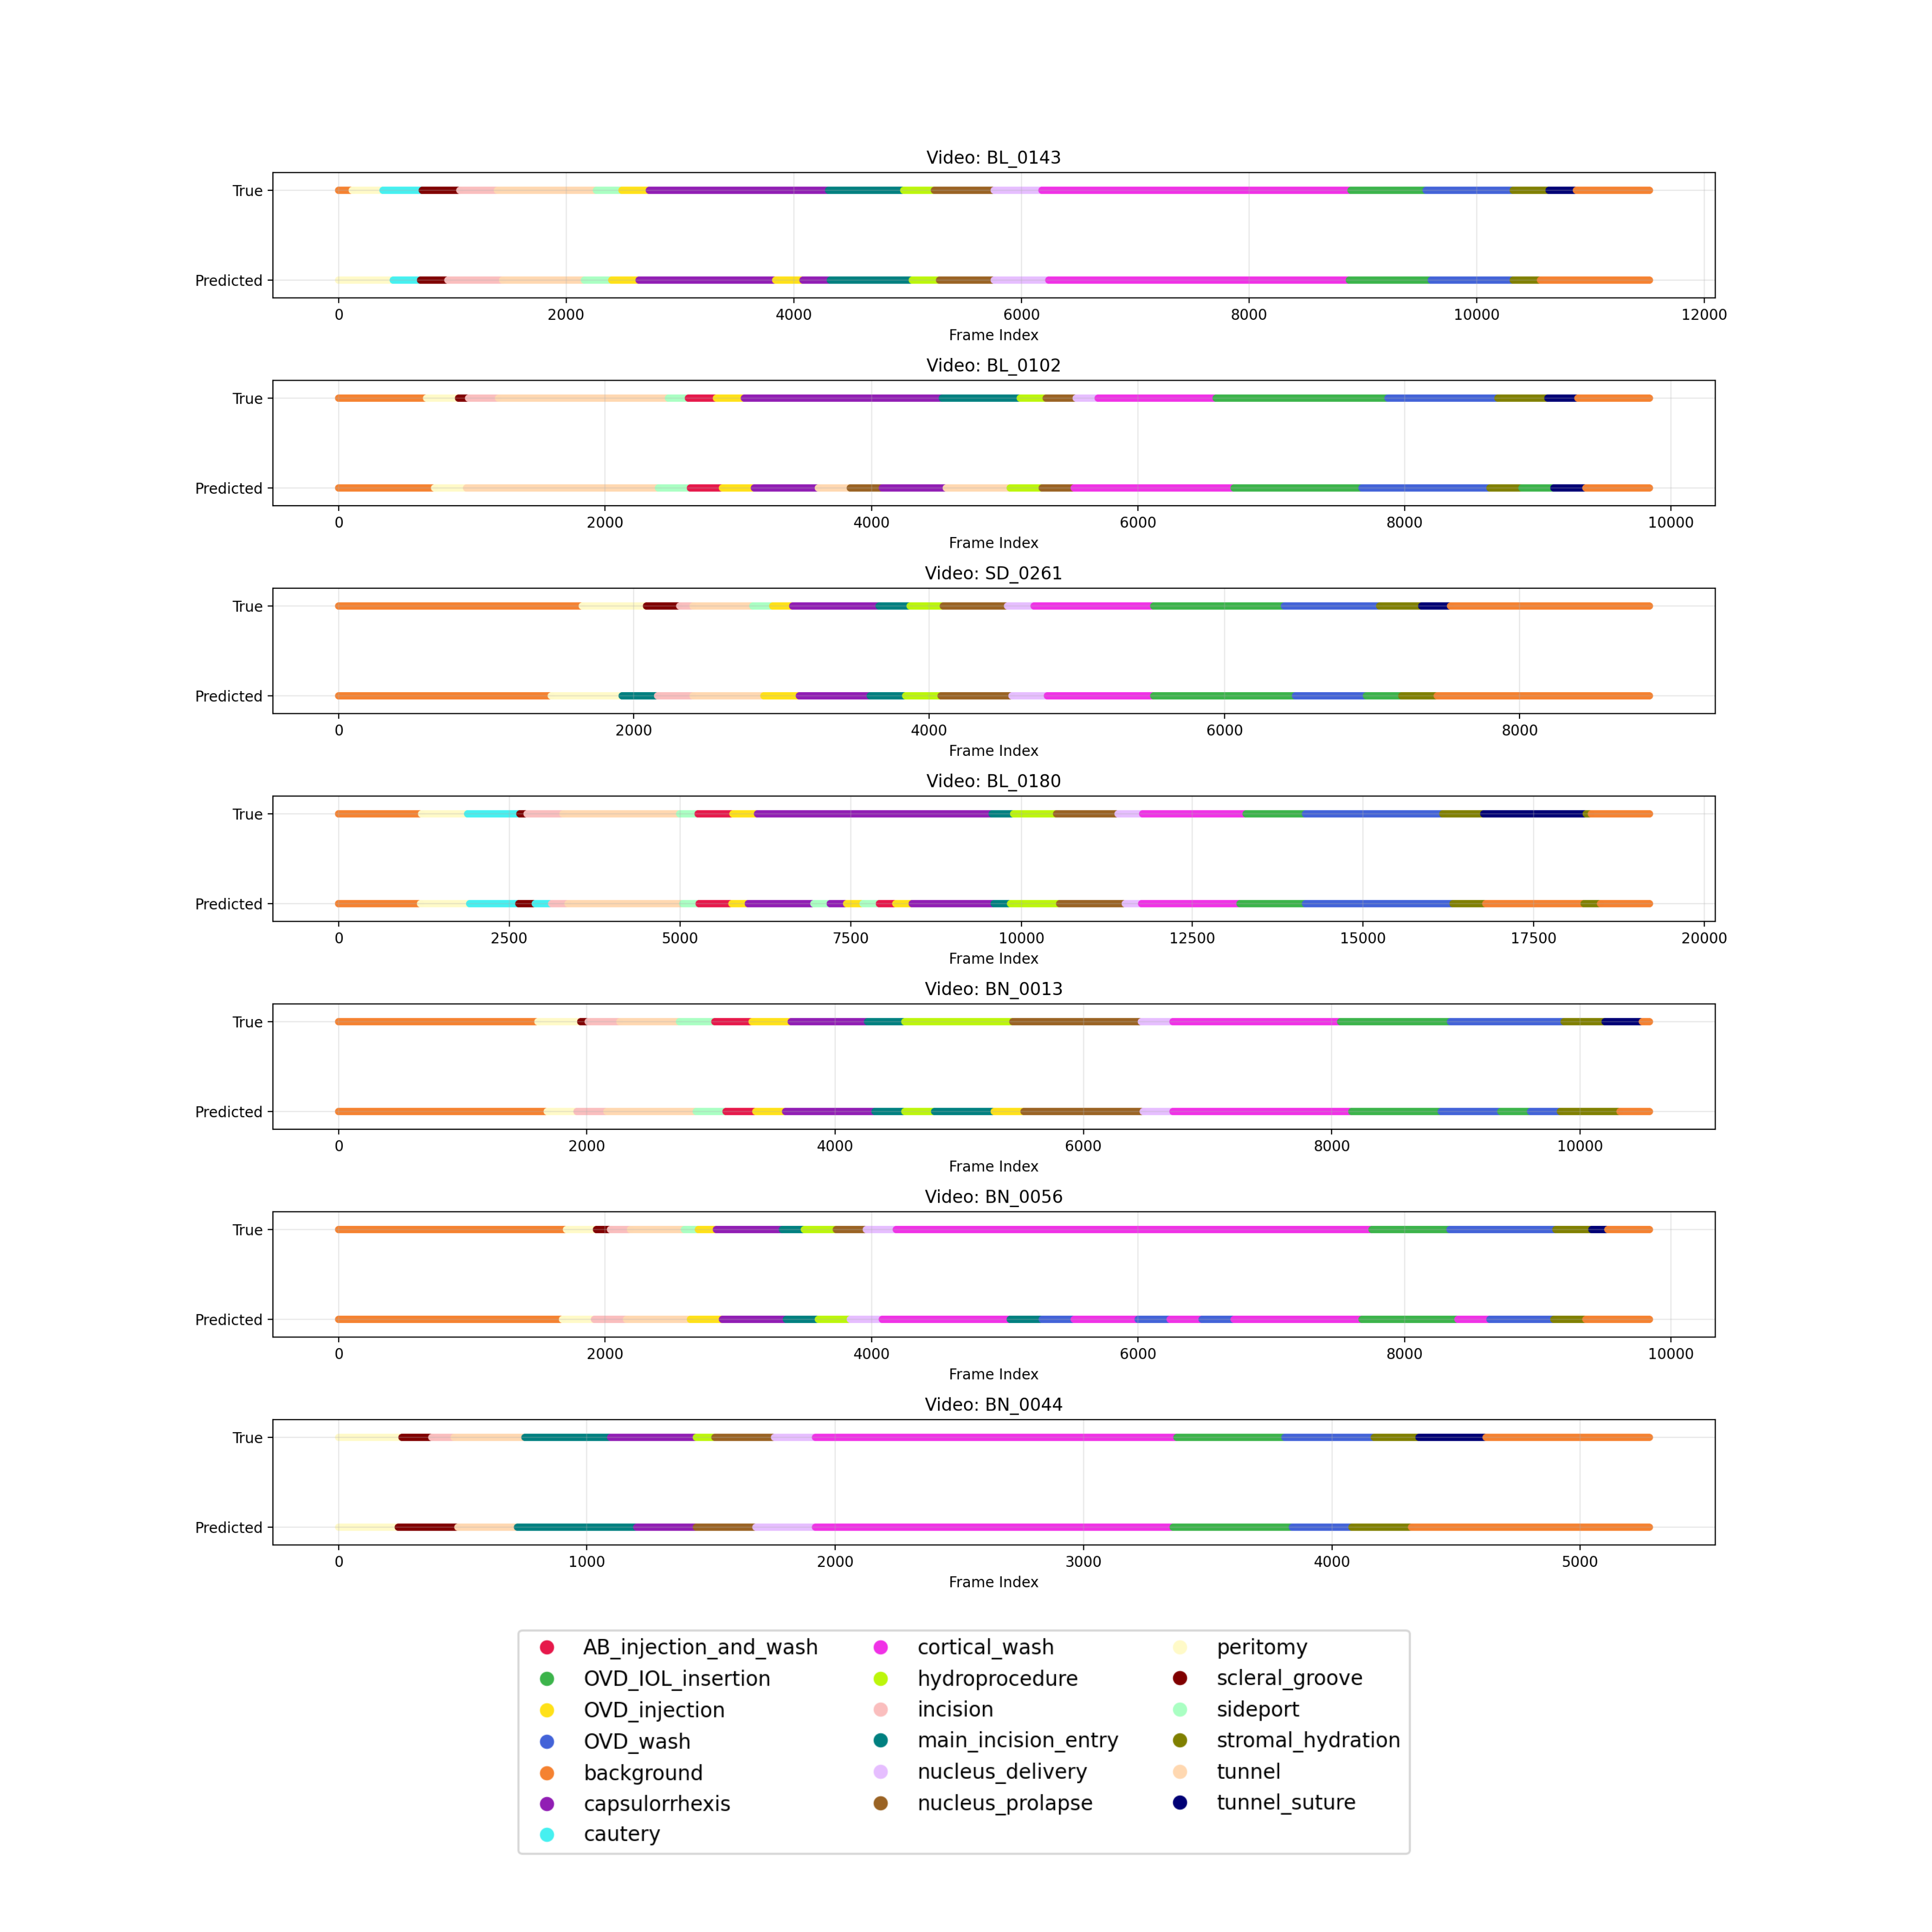
\includegraphics[width=\linewidth]{demo/images/merged_sequence.png}
%           \vspace{-2.0em}
%           \caption{\scriptsize Example sweep curves}
%           \vspace{-1.2em}
%         \end{figure}
%         \vspace{0.1em}
%       \end{block}
%   \end{columns}
% \end{frame}

% ========================================================
% Slide 8 — Qualitative Results
% ========================================================
\begin{frame}[label=slide8]{Qualitative Results}
  \begin{block}{}
    \vspace{-1.0em}
    \begin{figure}[H]
      \centering
      \vspace{-1.0em}
      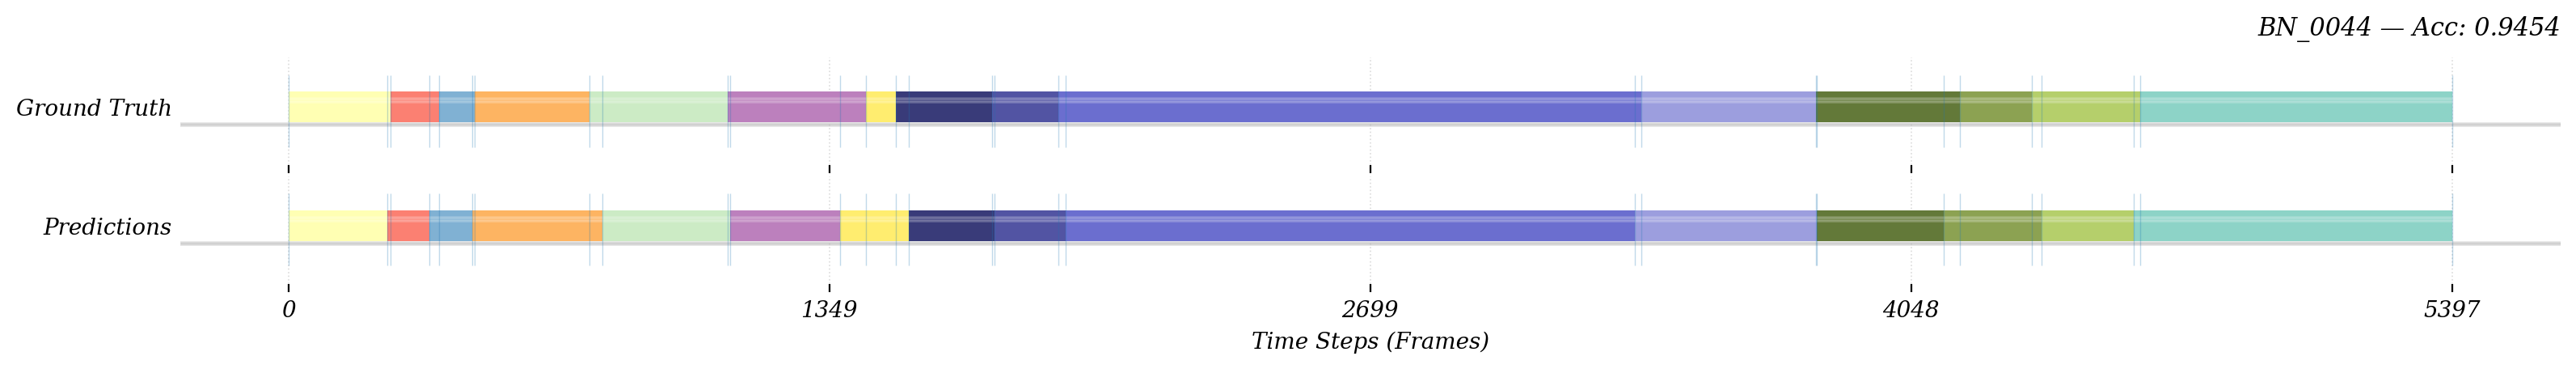
\includegraphics[width=0.8\linewidth]{demo/images/output_plot.png}
      \vspace{-2.0em}
      \caption{\scriptsize Ground truth (top) vs. predictions (bottom) showing cleaner boundaries and reduced over-segmentation}
      \vspace{-1.0em}
    \end{figure}
    \vspace{0.4em}
    \begin{figure}[H]
      \centering
      \vspace{-0.8em}
      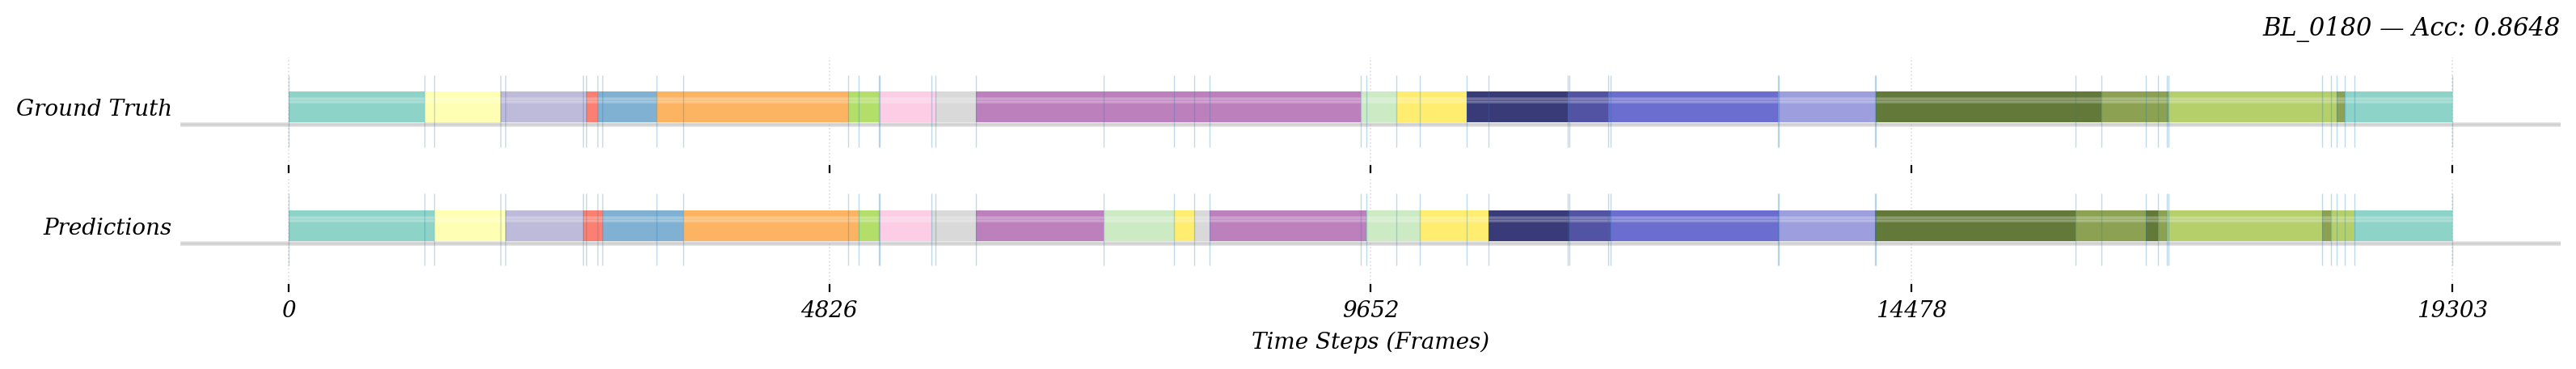
\includegraphics[width=0.8\linewidth]{demo/images/output2_plot.png}
      \vspace{-2.0em}
      \caption{\scriptsize Additional sequence showing consistent boundary alignment}
      \vspace{-1.0em}
    \end{figure}
    \vspace{0.1em}
  \end{block}
\end{frame}

% ========================================================
% Slide 9 — Ablation Study & Analysis
% ========================================================
\begin{frame}[label=slide9]{Ablation Study \& Analysis}
  \begin{columns}[T,onlytextwidth]
    \column{0.65\textwidth}
      \begin{block}{Component Analysis}
        \textbf{Boundary Head Impact:}
        \begin{itemize}
          \item BCE loss alone: marginal improvement
          \item Weighted TV loss alone: moderate improvement
          \item Combined: best performance (+1.3\% accuracy)
        \end{itemize}
        
        \textbf{Training Dynamics:}
        \begin{itemize}
          \item Warm start critical for stable convergence
          \item Learning rate $1 \times 10^{-4}$ optimal
          \item Higher rates cause training instability
        \end{itemize}
      \end{block}
      
      \begin{block}{Hyperparameter Sensitivity}
        \begin{itemize}
          \item $\gamma = 2.0$ optimal for TV exponent
          \item $\beta = 1.0$ best boundary loss weight
          \item Merge weight $w = 0.50$ most stable
        \end{itemize}
      \end{block}
      
    \column{0.3\textwidth}
      \begin{block}{Computational Cost}
        \textbf{Training:}
        \begin{itemize}
          \item +1 Conv1D per block
          \item Negligible parameter increase
        \end{itemize}
        
        \textbf{Inference:}
        \begin{itemize}
          \item Identical to baseline
          \item No runtime overhead
        \end{itemize}
      \end{block}
      
      \vspace{0.5em}
      \begin{block}{Limitations}
        \begin{itemize}
          \item Single dataset (SICS-155)
          \item I3D features only
          \item Binary boundary supervision
        \end{itemize}
      \end{block}
  \end{columns}
\end{frame}

% ========================================================
% Slide 10 — Conclusion & Future Work
% ========================================================
\begin{frame}[label=slide10]{Conclusion \& Future Work}
  \begin{columns}[T,onlytextwidth]
    \column{0.65\textwidth}
      \begin{block}{Key Contributions}
        \textbf{Methodological:}
        \begin{itemize}
          \item Strategic boundary head integration into \factmodel
          \item Boundary-weighted temporal smoothing loss
          \item Training-only overhead design
        \end{itemize}
        
        \textbf{Results:}
        \begin{itemize}
          \item 82\% accuracy on test set (Rank \#2)
          \item Qualitative reduction in over-segmentation
          \item Consistent gains with proper warm start
        \end{itemize}
      \end{block}
      
      \begin{block}{Clinical Impact}
        \begin{itemize}
          \item Better phase boundary detection for surgical training
          \item Improved quality assurance tools
          \item Cost-effective for resource-limited settings
        \end{itemize}
      \end{block}
      
    \column{0.3\textwidth}
      \begin{block}{Future Work}
        \begin{itemize}
          \item Alternative boundary integration strategies
          \item Cross-dataset generalization
          \item Real-time deployment optimization
          \item Clinical validation trials
        \end{itemize}
      \end{block}
  \end{columns}
  
  \vspace{0.5em}
  \begin{center}
    \begin{minipage}{0.8\textwidth}
      \centering
      \scriptsize
      \textbf{Boundary-aware training improves temporal consistency at no computational cost.}
    \end{minipage}
  \end{center}
\end{frame}

% ========================================================
% Thank You Slide
% ========================================================
\begin{frame}[standout]
  \begin{center}
    {\Huge Thank You}
    \vspace{1cm}
    
    \separator
    
    \vspace{0.5cm}
    
    \begin{columns}[T,onlytextwidth]
      \column{0.28\textwidth}
        \centering
        {\normalsize\textbf{Yasser El Jarida}\\
        UM6P College of Computing\\
        \texttt{yasser.eljarida@um6p.ma}}
      \column{0.28\textwidth}
        \centering
        {\normalsize\textbf{Youssef Iraqi}\\
        UM6P College of Computing\\
        \texttt{youssef.iraqi@um6p.ma}}
      \column{0.28\textwidth}
        \centering
        {\normalsize\textbf{Loubna Mekouar}\\
        UM6P College of Computing\\
        \texttt{loubna.mekouar@um6p.ma}}
    \end{columns}
    \vspace{2em}
    {\large Slides: \url{https://yasser.sh/talks/miccai_sics155/}}
  \end{center}
\end{frame}

\end{document}
